\documentclass[useAMS,usenatbib]{mn2e}
\bibliographystyle{mn2e}
\pdfoutput=1
\pdfminorversion=5

%\usepackage{widetext}
\usepackage{graphicx}
\usepackage{dcolumn}
\usepackage{bm}
\usepackage{amssymb,amsmath,bm}  
\usepackage{color}
\usepackage[colorlinks,linkcolor=red,citecolor=blue,urlcolor=blue ]{hyperref}
\usepackage{multirow}
\usepackage[utf8]{inputenc}
\usepackage{balance}
\usepackage{enumitem}
\usepackage{lipsum}
\newcommand{\nv}{\hat{\boldsymbol{\theta}}}
\newcommand{\wisc}{WI$\times$SC}
\newcommand{\TODO}[1]{{\bf TODO:} #1}
\newcommand{\todo}[1]{{\bf TODO:} #1}
\newcommand{\kalo}{Karhunen-Lo\`{e}ve\,}
\newcommand{\jcap}{JCAP}
\newcommand{\mnras}{MNRAS}
\newcommand{\aap}{A\&A}
\newcommand{\aaps}{A\&AS}
\newcommand{\apjs}{ApJS}
\newcommand{\apj}{ApJ}
\newcommand{\apjl}{ApJL}
\newcommand{\prd}{Phys.~Rev.~D}
\newcommand{\aj}{Astron. Journal}
\newcommand{\pasp}{Publications of the ASP}
\newcommand{\nar}{New Astronomy Review}
\newcommand{\procspie}{Proceedings of the SPIE}
\newcommand{\physrep}{Physics Reports}

\title[Tomographic measurement of the gas pressure through galaxy-tSZ cross-correlations]{Tomographic measurement of the gas pressure through galaxy-tSZ cross-correlations}
\author[David Alonso]{Nick Koukoufilippas$^1$, David Alonso$^1$, Maciej Bilicki$^2$, John A. Peacock$^3$\\
                      $^{1}$Department of Physics, University of Oxford, Keble Road, Oxford, OX1 3RH, UK\\
                      $^{2}$Center for Theoretical Physics, Polish Academy of Sciences, al. Lotnik\'ow 32/46, 02-668, Warsaw, Poland\\
                      $^{3}$Institute for Astronomy, University of Edinburgh, Royal Observatory, Edinburgh EH9 3HJ, United Kingdom
                      }

\begin{document}
  \date{\today}
  \pagerange{1--18} \pubyear{2018}
  \maketitle

\begin{abstract}
  \lipsum[1]
\end{abstract}

\begin{keywords}
  cosmology: large-scale structure of the Universe -- methods: data analysis
\end{keywords}

\section{Introduction}\label{sec:intro}
  Modern observational cosmology has reached a stage where the constraining power of most current and future datasets are limited by astrophysical systematic uncertainties, i.e. our lack of understanding of the physics behind the luminous components of the Universe, galaxies and gas \TODO{cites}, especially on the smallest scales. The limiting factor for cluster number counts is the uncertainty in the mass-observable relation. Cosmic shear measurements are strongly affected by sub-grid baryonic physics, and by uncertainties in the processes by which galaxies acquire correlated intrinsic alignments. Finally, even though the clustering pattern of galaxies is one of the cosmological observables with the highest signal-to-noise ratio, the cosmological constraints that can be extracted from it is severely limited by our lack of understanding of the galaxy-dark matter connection. Even the analysis of the temperature anisotropies in the Cosmic Microwave Background (CMB), arguably the cleanest cosmological observable, are currently limited by the impact of astrophysical foregrounds on small scales \TODO{cites everywhere}.
  
  The CMB secondary anisotropies, in particular the thermal and kinetic Sunyaev-Zel'dovich effects (tSZ and kSZ respectively), as well as the gravitational lensing of the CMB photons, have gained popularity as a means to address this issue \TODO{cite}. These effects are relatively clean probes of some of the physical quantities that need to be understood in order to mitigate the impact of astrophysical uncertainties: the matter and gas densities, the gas pressure and the velocity field. Since these observables are also sensitive to cosmology, their combination with large-scale structure data can be extremely powerful at disentangling astrophysical and cosmological parameters. This has been explored by a large number of groups: CMB lensing data has been used to constrain the bias of different tracers of the matter distribution \todo{cites}, as well as to calibrate the measurement of galaxy shapes in cosmic shear analyses \todo{cites}. The tSZ effect has been used in cross-correlation with galaxy clustering and weak lensing data to determine the physical properties of the diffuse gas, as well as to potentially improve constraints on the amplitude of matter fluctuations \todo{cites}. The kSZ in turn has been used in cross-correlation with galaxy clustering to constrain the growth of structure and the properties gas density profile around halos \todo{cites}.
  
  In this work we will focus on the cross-correlation between galaxy clustering data and maps of the tSZ Compton-$y$ parameter, making use of existing data from the Planck collaboration \todo{cites} and a set of photometric galaxy surveys. Several questions can be addressed through this combined analysis. Through tomography, this cross-correlation can be used to reconstruct the redshift evolution of the thermal gas pressure, as well as the dependence of the mass bias for tSZ cluster studies on redshift and, potentially, halo mass. This is a relevant topic given the current mild tensions between SZ cluster number counts and CMB primary anisotropies \todo{cites}, which could be caused by the assumptions made to model the $y$-mass relation. Conversely, under the assumption that the relation between mass and gas pressure is well understood, the tSZ effect can be thought of as a mass tracer, which can be used to break degeneracies with the galaxy bias parameter.

  This paper is structured as follows: Section \ref{sec:theory} presents the theoretical background used here to describe our two main observables, the projected overdensity of galaxies and the Compton-$y$ parameter, as well as their cross-correlation. Section \ref{sec:data} presents the datasets used for our analysis. The methods used to analyse these data are described in Section \ref{sec:methods}, and Section \ref{sec:results} presents the results. We summarize our conclusions in Section \ref{sec:discussion}.

\section{Theory}\label{sec:theory}
    Our analysis will focus on the cross-correlation of the projected galaxy overdensity in tomographic redshift bins $\delta_g$ and maps of the tSZ Compton-$y$ parameter.
    
    $\delta_g$ is simply the overdensity in the number of galaxies integrated over a redshift bin:
    \begin{equation}
      \delta_g(\nv)=\int dz\,\phi_g(z)\,\Delta_g(\chi(z)\,\nv),
    \end{equation}
    where $\nv$ is a unit vector on the sphere, $\chi(z)$ is the comoving radial distance to redshift $z$ and $\phi_g(z)$ is the normalized galaxy redshift distribution in the bin. $\Delta_g({\bf x})=n_g({\bf x})/\bar{n}_g-1$ is the 3D galaxy overdensity, where $n_g$ is the galaxy number density.
    
    The Compton-$y$ parameter in turn is given by \todo{cite}:
    \begin{equation}
      y(\nv)=\frac{\sigma_T}{m_ec^2}\int \frac{d\chi}{(1+z)} P_e(\chi\nv),
    \end{equation}
    where $P_e=n_e\,T_e$ is the electron pressure ($n_e$ and $T_e$ are the electron density and temperature respectively), $\sigma_T$ is the Thomson scattering cross-section, and $m_e$ is the electron mass.
    
  \subsection{Projected fields and angular power spectra}\label{ssec:theory.cls}    
    Both $\delta_g$ and $y$ can be described as a projected quantity $u(\nv)$ related to a three-dimensional field $U({\bf r})$ through some radial kernel $W_u(\chi)$:
    \begin{equation}
      u(\nv)=\int d\chi\,W_u(\chi)\,U(\chi\nv).
    \end{equation}
    Any projected quantity can be decomposed into its spherical harmonic coefficients $u_{\ell m}$, the covariance of which is the so-called angular power spectrum $\langle u_{\ell m}v^*_{\ell' m'}\rangle\equiv C^{uv}_\ell\delta_{\ell\ell'}\delta_{mm'}$.

    The angular power spectrum can be related to the 3D power spectrum of the associated 3D fields $P_{UV}$ as\footnote{Note that Eq. \ref{eq:cllimber} is only valid in the {\sl Limber approximation} \todo{cite}, which is accurate for broad radial kernels. This approximation is adequate for the redshift distributions used here.}:
    \begin{equation}\label{eq:cllimber}
      C_\ell^{uv} = \int d\chi \frac{W_u(\chi)W_v(\chi)}{\chi^2}\,P_{UV}\left( z, k=\frac{\ell+1/2}{\chi} \right).
    \end{equation}
    Here, the 3D power spectrum is analogously defined as the variance of the Fourier-space 3D quantities:
    \begin{equation}
      \left\langle U({\bf k})V^*({\bf k}')\right\rangle = (2\pi)^3\,\delta({\bf k}-{\bf k}')\,P_{UV}(k).
    \end{equation}
    We will model the 3D power spectrum using the halo model described in \ref{ssec:theory.hm} below.

    In this formalism, the 3D quantities associated to $\delta_g(\nv)$ and $y(\nv)$ are the 3D overdensity $\Delta_g({\bf x})$ and the electron pressure $P_e({\bf x})$ respectively. The associated radial kernels are:
    \begin{equation}
      W_g(\chi)=\frac{H(z)}{c}\,\phi_g(z),\hspace{12pt}W_y(\chi)=\frac{\sigma_T}{m_ec^2}\frac{1}{1+z},
    \end{equation}
    where $H(z)$ is the expansion rate.

  \subsection{Halo model predictions}\label{ssec:theory.hm}
    The halo model \TODO{cite} describes the spatial fluctuations of any quantity in terms of the contributions to it of all dark matter haloes, under the assumption that all the matter in the Universe is contained in those haloes. We will only quote here the final results regarding the halo model prediction for power spectra, and refer the reader to \TODO{cite} for further details.
    
    Let $U(r|M)$ be the profile of a given quantity as a function of the comoving distance $r$ to the centre of a halo of mass $M$, and let $U(k|M)$ be its Fourier transform:
    \begin{equation}
      U(k|M)\equiv4\pi \int_0^\infty dr\,r^2\,\frac{\sin(kr)}{kr}U(r|M).
    \end{equation}

    The halo model prediction for the cross-power spectrum $P_{UV}$ then consists of two contributions, from the so-called 1-halo term and 2-halo term:
    \begin{equation}
      P_{UV}(k)=P^{1h}_{UV}(k)+P^{2h}_{UV}(k).
    \end{equation}
    Each of these can be estimated in terms of the Fourier-space profiles as:
    \begin{align}
      &P^{1h}_{UV}(k)=\int dM\,\frac{dn}{dM}\,\langle U(k|M)\,V(k|M)\rangle,\\
      &P^{2h}_{UV}(k)=\langle bU\rangle\,\langle bV\rangle\,P_L(k),\\
      &\langle bU\rangle(k)\equiv\int dM\frac{dn}{dM}\,b_h(M)\,\langle U(k|M)\rangle. \label{eq:hm_bias}
    \end{align}
    Here, $P_L(k)$ is the linear matter power spectrum, $dn/dM$ is the halo mass function and $b_h(M)$ is the halo bias \TODO{cites}. %Further details are discussed in Appendix \ref{app:hm}.
    
    \TODO{describe $1h$-$2h$ transition correction.}
    
    \subsubsection{Galaxies and the halo occupation distribution}\label{sssec:theory.hm.hod}
      To model the galaxy overdensity $\Delta_g$ we will use a Halo Occupation Distribution (HOD) model \cite{2002ApJ...575..587B,2005ApJ...633..791Z,2013MNRAS.430..725V}, as prescribed by \cite{2011ApJ...736...59Z}. The HOD models the galaxy content of dark matter halos as being made up of central and satellite galaxies. Centrals lie at the center of the halo, while satellites are distributed according to a profile $u_s(r|M)$. Halos can have zero or one central, and the mean number of centrals for a halo of mass $M$ is modelled as a smoothed step function
      \begin{equation}
        \langle N_c(M)\rangle=\frac{1}{2}\left[1+{\rm erf}\left(\frac{\log(M/M_{\rm min})}{\sigma_{\rm lnM}}\right)\right].
      \end{equation}
      We then assume that satellites can only be formed if a halo has a central and has a mass larger than some threshold $M_0$. In that case, average number of satellites is a power law of the form:
      \begin{equation}
        \langle N_s(M)\rangle=\Theta(M-M_0)\,\left(\frac{M-M_0}{M_1'}\right)^{\alpha_s}.
      \end{equation}
      For simplicity, we will fix $M_0$ to $M_{\rm min}$, $\sigma_{\rm lnM}=0.15$ and $\alpha_s$=1 \cite{2018MNRAS.473.4318A}, leaving only two free parameters: $M_{\rm min}$ and $M_1'$.
      
      Besides their mean values, we also need to specify the statistics of $N_c$ and $N_s$. Following the standard practice \cite{2013MNRAS.430..725V}, we assume $N_c$ to have a binomial distribution with probability $p=\langle N_c\rangle$, and $N_s$ to be Poisson-distributed.

      Putting everything together, the moments of the galaxy overdensity Fourier profile are \cite{2013MNRAS.430..725V}:
      \begin{align}
        &\langle u_g(k)\rangle=\bar{n}_g^{-1}\langle N_c\rangle\left[1+\langle N_s\rangle\,u_s(k)\right],\\
        &\langle |u_g(k)|^2\rangle=\bar{n}_g^{-2}\langle N_c\rangle\left[\langle N_s\rangle^2u_s^2(k)+2\langle N_s\rangle u_s(k)\right],
      \end{align}
      where the mean number density $\bar{n}_g$ is
      \begin{equation}
        \bar{n}_g\equiv\int dM\,\frac{dn}{dM}\langle N_c\rangle\left[1+\langle N_s\rangle\right],
      \end{equation} 
      and we have suppressed the mass dependence of all quantities for simplicity.

      Finally, we will assume that the satellites follow the matter distribution, and therefore $u_s(k|M)$ is given by a truncated Navarro-Frenk and White profile \cite{1996ApJ...462..563N}:
      \begin{align}
        u_s(k|M)=&\left[\log(1+c_\Delta)-\frac{c_\Delta}{(1+c_\Delta)}\right]^{-1}\\
               &\left[\cos(q)\left({\rm Ci}((1+c_\Delta)q)-{\rm Ci}(q)\right)\right.\\\nonumber
               &\left.+\sin(q)\left({\rm Si}((1+c_\Delta)q)-{\rm Si}(q)\right)\right.\\&\left.-\sin(c_\Delta q)/(1+c_\Delta q)\right],
      \end{align}
      where $q\equiv kr_\Delta/c_\Delta$, $r_\Delta$ and $c_\Delta$ are the halo radius and concentration defined in Section \ref{sssec:theory.hm.cm}, and $\{{\rm Ci}, {\rm Si}\}$ are the cosine and sine integrals.
      
    \subsubsection{tSZ and pressure profiles}\label{sssec:theory.hm.pe}
      In order to describe the electron pressure in a halo, we use the generalized NFW profile (GNFW) described in \cite{2010A&A...517A..92A} and used in the Planck tSZ cluster analysis \cite{2016A&A...594A..24P}. This profile takes the form:
      \begin{equation}
        P_e(r)=P_*\,p(r/r_{500c}),
      \end{equation}
      where $r_{500c}$ is the cluster radius enclosing an overdensity of 500 times the critical density (see Section \ref{sssec:theory.hm.cm}). The normalization $P_*$ is given by
      \begin{equation}
        P_*=6.41\,\left(1.65 {\rm eV}\,{\rm cm}^{-3}\right)h_{70}^{8/3}
        \left(\frac{h_{70}(1-b_H)M_{500c}}{3\times10^{14}M_\odot}\right)^{0.79},
      \end{equation}
      where $h_{70}=H_0/(70 {\rm km}\,{\rm s}^{-1}\,{\rm Mpc}^{-1}$, and $(1-b_H)$ is the so-called m bias parameter. The GNFW form factor is
      \begin{equation}
        p(x)=(c_P x)^{-\gamma}\left[1+(c_P x)^\alpha\right]^{(\gamma-\beta)/\alpha},
      \end{equation}
      with $(\alpha,\beta,\gamma,c_P)=(1.33,4.13,0.31,1.81)$.
      
      \TODO{Blah about $(1-b_H)$}. Other pressure profiles have been proposed in the literature (e.g. \cite{2012ApJ...758...75B}), but we choose this parametrisation in order to be able to relate our measurement of $(1-b_H)$ to the results of \cite{2016A&A...594A..24P}.
      
      Within the halo model description, and assuming a log-normal $y$-mass relation, the pressure profile cumulants are given by:
      \begin{align}
        &\langle u_y(k|M)\rangle=P_e(k),\\
        &\langle u_y^2(k|M)\rangle=P_e^2(k)\,e^{\sigma_{\ln Y}^2},
      \end{align}
      where $P_e(k)$ is the Fourier transform of the GNFW profile and $\sigma_{\ln Y}=0.173\pm0.023$ is the intrinsic logarithmic scatter in the $y$-mass relation \cite{2016A&A...594A..24P}. Note that, since we do not make use of the tSZ auto-correlation, we will not use the second order cumulant of the pressure profile in our analysis. However, since we analyse the galaxy-tSZ correlation, we need to model the covariance between the galaxy overdensity and pressure profiles. For simplicity, we adopt a simple parametrization:
      \begin{equation}
        \langle u_y(k|M) u_g(k|M)\rangle = (1+\rho_{yg})\langle u_g(k|M)\rangle \langle u_y(k|M)\rangle,
      \end{equation}
      where $\rho_{yg}$ is a free parameter that determines the sign of the correlation between galaxy abundance and pressure. Marginalising over this parameter has the added advantage of reducing the sensitivity of our final constraints on $1-b_H$ on the details of the cross-spectrum model in the 1-halo regime, where both parameters are completely degenerate.

      It is also worth exploring the halo model bias (Eq. \ref{eq:hm_bias}) for the Compton-$y$ paramete. At $k\rightarrow0$ this is given by:
      \begin{align}\nonumber
        \langle bP_e\rangle&=\int dM\,\frac{dn}{dM}\,b_h(M)\,\int_0^\infty dr\,4\pi r^2\,P_e(r|M)\\
               &=\int dM\,\frac{dn}{dM}\,b_h(M)\,E_T(M),
      \end{align}
      where $E_T(M)$ is the thermal energy in a halo of mass $M$ \cite{2017MNRAS.467.2315V,2019arXiv190413347P}. A measurement of $\langle bP_e\rangle$ can be related to the thermodynamics of gas inside halos.
      
    \subsubsection{Concentration-mass relation and mass definitions}\label{sssec:theory.hm.cm}
      Halo radii $r_\Delta$ are usually defined as the size of the sphere containing a given mass $M_\Delta$:
      \begin{equation}
        M_\Delta = \frac{4\pi}{3}\rho_*(z)\Delta r^3_\Delta.
      \end{equation}
      Common choices for $\rho_*$ are the critical density $\rho_c=3H^2(z)/4\pi G$ and the matter density $\rho_M(z)$. The spherical overdensity parameter $\Delta$ is usually chosen within the range $\sim(200,500)$ and sometimes defined as the quantity yielding the virial radius in the spherical top-hat collapse model $\Delta_v$ \cite{1998ApJ...495...80B} \TODO{more refs?}.

      Ideally we would like to use the same mass definition (i.e. choice of $\Delta$ and $\rho_*$) for the mass function, the mass-concentration relation $c_\Delta(M)$ and the calibrated pressure profile. Unfortunately while the GNFW profile is calibrated to $\Delta_{500c}$ (where $c$ denotes critical density), the mass functions of \cite{2008ApJ...688..709T,2010ApJ...724..878T} are only provided for $\rho_M$-based mass definitions, and the concentration-mass relation of \cite{2008MNRAS.390L..64D} was only estimated for $\Delta=200$ (for critical and matter densities) and for $\Delta=\Delta_v$. To overcome this issue, we follow the procedure used by \cite{2016A&A...594A..24P} and \cite{2018MNRAS.477.4957B}: our baseline mass definition is $\rho_c$-based with $\Delta=500$, as used by \cite{2010A&A...517A..92A}. At each redshift, we translate this into a $\Delta$ value for a $\rho_M$-based definition, which we use to compute the mass function from the parametrizations of \cite{2008ApJ...688..709T,2010ApJ...724..878T}. We also rederive the concentration-mass relation of \cite{2008MNRAS.390L..64D} for a $\rho_c$-based $\Delta=500$ from their $\Delta=200$ parametrization by integrating the NFW profile to the corresponding halo radius. Within the redshifts covered by our analysis we find that this is well fit by:
      \begin{equation}
        c_{500c}(M,z)= A\,(M/M_{\rm pivot})^B\,(1+z)^C,
      \end{equation}
      with $M_{\rm pivot}=2.7\times10^{12}\,M_\odot$ and $(A,B,C)=(3.67,\,-0.0903,\,-0.51)$.

\section{Data}\label{sec:data}
  \subsection{The Compton-$y$ map}\label{ssec:data.y}
    \begin{figure}
      \centering
      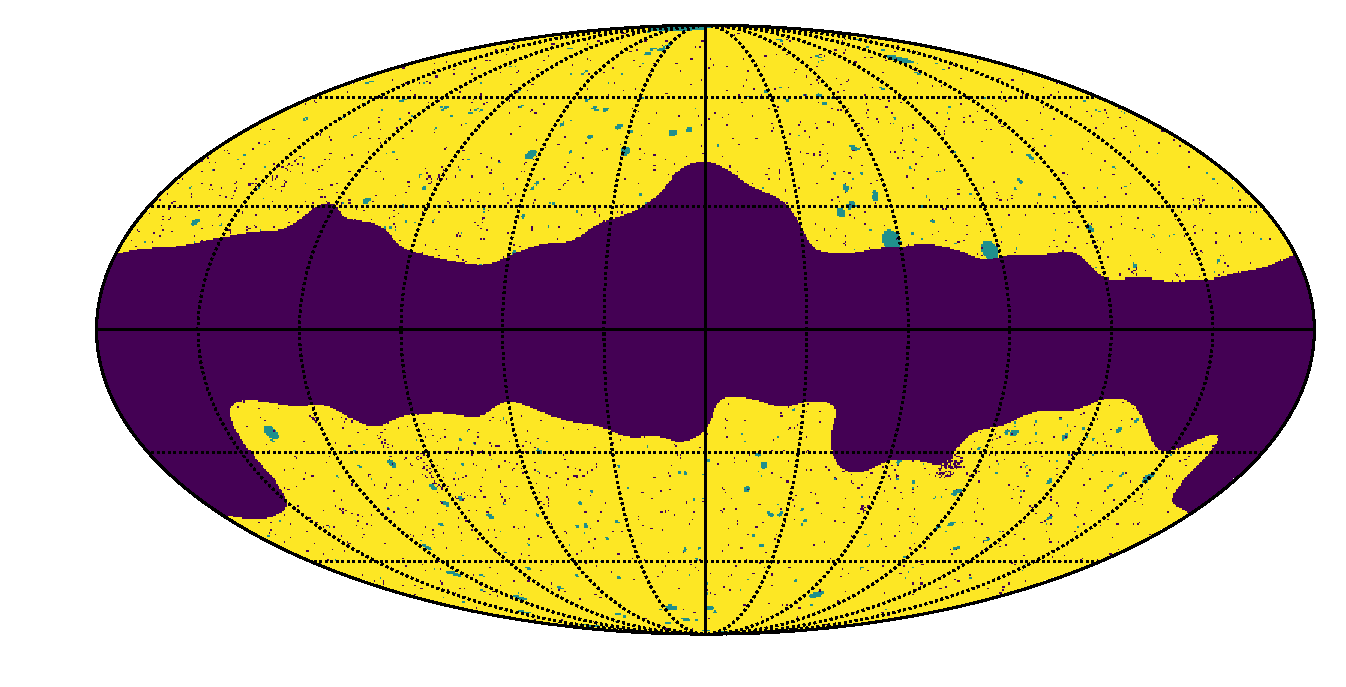
\includegraphics[width=0.5\textwidth]{./figures/mask_y.pdf}
      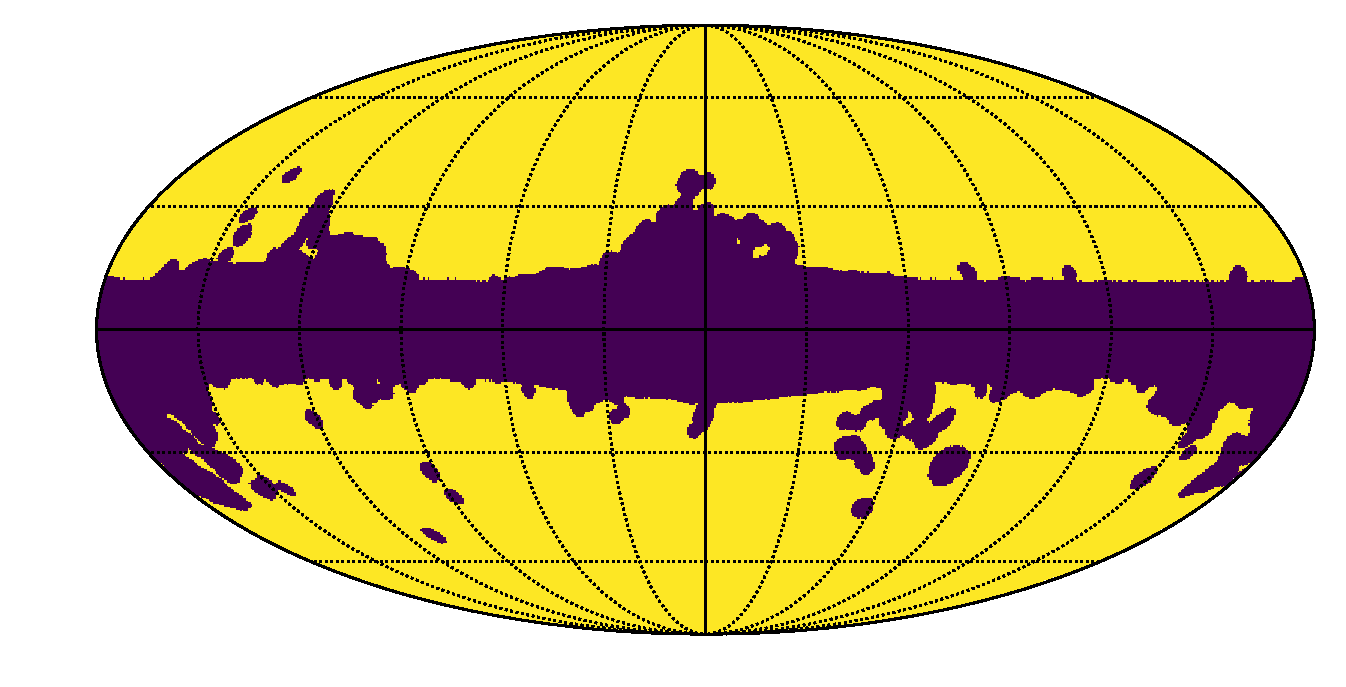
\includegraphics[width=0.5\textwidth]{./figures/mask_g.pdf}
      \caption{Sky masks used for the Compton-$y$ map (top) and for the 2MPZ and \wisc galaxy surveys (bottom). The top panel shows, in turquoise, the regions masked additionally when removing sky patches around the position of the tSZ sources detected by Planck above 6$\sigma$.}
      \label{fig:msk}
    \end{figure}
    We make use of the maps of the Compton-$y$ parameter made public by the Planck collaboration \cite{2016A&A...594A..22P}. These maps were generated using different flavours of the Internal Linear Combination method \cite{2004ApJ...612..633E,2008arXiv0811.4277V}. In a simplified description, the ILC technique selects the linear combination of all frequency channels that preserves the spectrum of the source one wishes to map minimizing the map-level variance. The refined versions of the ILC method used by Planck further optimize the linear weights on different scales and different regions of the map, and project out sources with known spectra that are likely to cause significant contamination. In particular, the Planck collaboration has released two $y$ maps, extracted using the MILCA \citep{2013A&A...558A.118H} and NILC \cite{2011MNRAS.410.2481R} variations of the ILC technique. Both methods deproject CMB contamination through its well-known spectrum, but differ on the methods used to calculate the optimal scale-dependent and spatially-varying linear weights.
    
    The MILCA and NILC maps have been found to be in good agreement in different studies \citep{2016A&A...594A..22P}, although the NILC map has a higher noise level on large scales \citep{2016A&A...594A..22P}. We thus use the MILCA map as our fiducial Compton-$y$ map, but will repeat our analysis on the NILC map as part of our systematics analysis.
    
    We use a fiducial mask for the $y$ maps based on a combination of the Planck 60\% Galactic mask and the union of the HFI and LFI point source masks. As part of our study of the mass dependence of the signal on halo mass, we additionally mask out all tSZ sources detected by Planck above 6$\sigma$, based on the Union catalog of \cite{2016A&A...594A..27P}.
    
    Finally, in order to evaluate the level of contamination from extragalactic dust in the $\delta_g$-$y$ correlation, we make used of the HFI 545 GHz map, as described in Section \ref{sssec:results.syst.y}.
    
  \subsection{2MPZ and \wisc}\label{ssec:data.g1}
    \begin{figure}
      \centering
      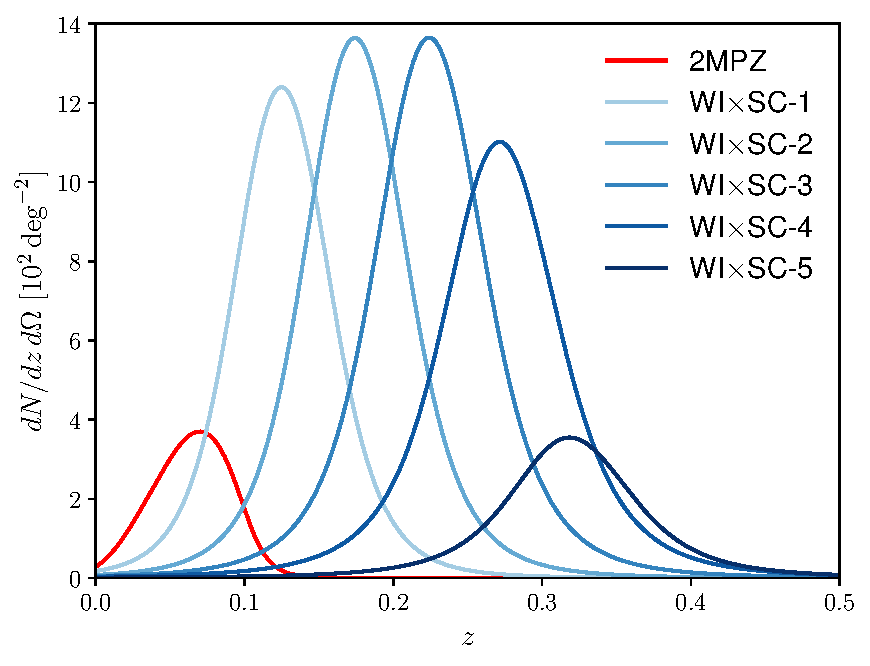
\includegraphics[width=0.5\textwidth]{./figures/nzs.pdf}
      \caption{Fiducial redshift distributions of the different galaxy samples used in this analysis. See Table \ref{tab:z_bins} for further details.}
      \label{fig:dndz}
    \end{figure}
    \begin{table}
      \begin{center}
        \begin{tabular}{l|ccc}
          \hline
          Sample & $[z_{{\rm ph},i},z_{{\rm ph},f}]$ & $\bar{z}$ & $\bar{n}_g\,[{\rm deg}^{-2}]$\\
          \hline
          2MPZ    & N.A.         & 0.07 &  25.5 \\
          \wisc-1 & $[0.1,0.15]$ & 0.13 & 106   \\
          \wisc-2 & $[0.15,0.2]$ & 0.18 & 126   \\
          \wisc-3 & $[0.2,0.25]$ & 0.23 & 136   \\
          \wisc-4 & $[0.25,0.3]$ & 0.27 & 118   \\
          \wisc-5 & $[0.3,0.35]$ & 0.32 & 41    \\
          \hline
        \end{tabular}
        \caption{Galaxy samples used in this analysis, corresponding to the full 2MPZ survey and five tomographic redshift bins of the \wisc survey. The second, third and last columns list the photometric redshift interval defining the sample, its mean redshift and its number density respectively.}\label{tab:z_bins}
      \end{center}
    \end{table} 
    We make use of two low-redshift photometric redshift catalogs, the 2MASS photometric redshift survey (2MPZ; \cite{2014ApJS..210....9B}) and the WISE $\times$ SuperCOSMOS catalogue (\wisc; \cite{2016ApJS..225....5B}). Both surveys were creating by cross-matching full-sky imaging surveys, and their broad photometric coverage allows them to achieve excellent photo-$z$ uncertainties.
    
    2MPZ was constructed by cross-matching the extended-source catalog from the 2 Micron All-Sky Survey (2MASS; \citep{2006AJ....131.1163S,2000AJ....119.2498J}) with the photographic plates of SuperCOSMOS \cite{2001MNRAS.326.1295H,2016MNRAS.462.2085P} and the photometry of the Wide-field Infrared Survey Explorer (WISE; \cite{2010AJ....140.1868W}). After applying an apparent magnitude cut $K_s<13.9$ to achieve uniformity, 2MPZ include over 940,000 sources observed in 8 bands: SuperCOSMOS's optical $(B,R,I)$, 2MASS's near-infrared $(J,H,K_s)$ and WISE's mid-infrared $(W1,W2)$. Photometric redshifts (photo-$z$s) were extracted using the neural network code ANNz \cite{2004PASP..116..345C} trained on a large spectroscopic sample from overlapping surveys. The resulting photo-$z$s have a typical error $\sigma_z\simeq0.015$, and the sample has a median redshift $z\sim0.08$. As we will see, due to the low redshift of this sample, the cross-correlation with the $y$ map is dominated by the 1-halo term for 2MPZ, and little is gained by sub-dividing it into narrow redshift bins. Therefore we use 2MPZ as a single tomographic sample.
    
    A deeper sample can be achieved by dropping the 2MASS data and cross-matching WISE and SuperCOSMOS only. After removing the sources already contained in 2MPZ, the resulting catalog, \wisc, is $\sim$3 times deeper, contains $\sim20$ million sources and reaches up to redshift $z\sim0.4$, with a median redshift of $\sim0.2$. The photometric redshifts are less accurate, given the poorer photometric coverage $(B,\,R,\,W1,\,W2)$, with a mean error $\sigma_z/(1+z)\simeq0.035$. We divide the \wisc sample into 5 redshift bins, corresponding to photo-$z$ intervals of equal width $\delta z_{\rm photo}=0.05$ in the range $0.1<z_{\rm photo}<0.35$. We estimate fiducial redshift distribution for each tomographic sample as described in \cite{2018MNRAS.481.1133P}, and we discuss the marginalization over uncertainties in these distributions in Section \ref{sssec:methods.syst.photoz}.

    Both 2MPZ and WISC suffer from contamination from Galactic and observational systematics in different levels. The most relevant Galactic systematic is star contamination, particularly for \wisc \cite{2018arXiv181208182X}. Besides avoiding regions of high dust and star contamination using the sky mask described in \cite{2018MNRAS.481.1133P}, we correct for the effects of stellar contamination by correcting for a smooth non-linear relation between galaxy and star density (also described in \cite{2018MNRAS.481.1133P}). After doing so, three potential sources of systematic uncertainty remain: residual stellar contamination, modulation of the galaxy density due to Galactic dust reddening and modulation due to zero-point fluctuations in the photographic plates used by SuperCOSMOS. We address the first two (dust and stars) by deprojecting them at the map level as described in Section \ref{sssec:methods.syst.deproj}. We address the contamination from fluctuations in the SuperCOSMOS plates by modelling it at the power spectrum level, which we describe in Section \ref{sssec:methods.syst.plates}.

\section{Methods}\label{sec:methods}
  \subsection{Estimating power spectra}\label{ssec:methods.cls}
    We measure all auto- and cross-power spectra between the different redshift bins and the $y$ maps using the pseudo-$C_\ell$ estimator \TODO{cites} as implemented in \TODO{cite}. Details about the method can be found in \TODO{cite}, but we provide a brief description here for completeness. For an incomplete sky coverage, a given field observed on the sphere, $\tilde{u}(\nv)$, can be modelled as a product of the true underlying field $u$, and a sky mask $w$
    \begin{equation}
      \tilde{u}^{\rm obs}(\nv) = w(\nv)\,u(\nv).
    \end{equation}
    In the simplest scenario, the mask $w$ is simply a binary map ($w=0$ or 1) selecting the pixels in the sky that have been observed. More generally, $w$ can be designed to optimally up- or downweight different regions in an inverse-variance manner. Through the convolution theorem, the spherical harmonic transform of the observed field is a convolution of the harmonic transforms of the true field and the mask. This then translates into a similar result for the ensemble average of the observed power spectra $\tilde{C}^{uv}_\ell$:
    \begin{equation}
      \tilde{C}^{uv}_\ell = \sum_{\ell'}\,M^{uv}_{\ell \ell'}\, C^{uv}_{\ell'},
    \end{equation}
    where $C^{uv}_\ell$ is the true underlying power spectrum. $M^{uv}_{\ell \ell'}$ is the so-called mode-coupling matrix, which depends solely on the masks of both fields, and which can be computed analytically. Roughly speaking, the pseudo-$C_\ell$ approach is then based on estimating $M^{uv}$ and inverting it to yield an unbiased estimate of the power spectrum.
    
    For the galaxy auto-correlation, the pseudo-$C_\ell$ method requires an additional step of subtracting the shot noise bias. We do so analytically following the approach described in Section 2.4.2 of \TODO{cite} with a local noise variance given by $\sigma_n^2=1/\bar{n}_\Omega$, where $\bar{n}_\Omega$ is the mean surface number density in units of ${\rm sr}^{-2}$.

  \subsection{Covariance matrices}\label{ssec:methods.cov}
    We combine two different methods to estimate the power spectrum covariance matrix. 
    
    We make a first estimate of the covariance using the jackknife resampling method. We divide the common footprint covered by the masks of both the galaxy overdensity and Compton-$y$ maps into $N_{\rm JK}$ regions with roughly equal area. We mask out each region in turn and compute the power spectrum  using the remaining available footprint. The covariance matrix is then estimated as:
    \begin{equation}
      {\rm Cov}\left(C^{uv}_\ell,C^{wz}_{\ell'}\right)=\frac{N_{\rm JK}-1}{N_{\rm JK}}\sum_{n=1}^{N_{\rm JK}}\Delta C^{uv,(n)}_\ell\,\Delta C^{wz,(n)}_{\ell'},
    \end{equation}
    where $\Delta C^{uv,(n)}_\ell$ is the difference between the power spectrum estimated when removing the $n$-th jackknife region and the power spectrum averaged over all jackknife regions. We use 461 jackknife regions defined as {\tt HEALPix} pixels with resolution $N_{\rm side}=8$.

    Although the jackknife method is able to provide an estimate of the size of the power spectrum uncertainties in a model independent way, it also has its drawbacks. There are only so many jackknife regions that can be selected with a reasonable size, and therefore the estimated covariance is noisy at some level. Furthermore, since the footprint associated with the removal of each jackknife region is different from the overall footprint, the method is also not able to recover the mode-coupling associated with the map geometry by construction. In order to verify and improve our estimate of the covariance matrix, we make use of a second analytical estimator.

    We compute the analytical covariance matrix following the methods outlined in \TODO{cite}. The covariance receives two main additive contributions, from the so-called {\sl disconnected} and {\sl connected} trispectra. The disconnected part is essentially the covariance matrix estimated under the assumption that all fields are Gaussianly distributed. In the absence of sky masks, it is given by
    \begin{equation}
      {\rm Cov}^{\rm G}\left(C^{uv}_\ell,C^{wz}_{\ell'}\right)=\delta_{\ell\ell'}\frac{C^{uw}_\ell C^{vz}_\ell+C^{uz}_\ell C^{vw}_\ell}{2\ell+1}.
    \end{equation}
    A sky mask introduces non-zero coupling between different $\ell$ modes. To account for these, we use the  method introduced in \TODO{cite}, which has been shown to be an excellent approximation for large-scale structure data \TODO{cite}.

    We compute the connected (i.e. non-Gaussian) contribution to the covariance matrix using the halo model as the 1-halo trispectrum \TODO{cite}, given by:
    \begin{align}\nonumber
      {\rm Cov}^{\rm NG}\left(C^{uv}_\ell,C^{wz}_{\ell'}\right)=\int &d\chi\,\frac{W_u(\chi)W_v(\chi)W_w(\chi)W_z(\chi)}{4\pi f_{\rm sky}\,\chi^6}\times\\\label{eq:cov_ng}
      &T^{1h}_{uvwz}\left(k=\frac{\ell+1/2}{\chi}\right),
    \end{align}
    where
    \begin{equation}\nonumber
      T^{1h}_{uvwz}(k)\equiv\int dM\frac{dn}{dM}\langle U(k|M) V(k|M) W(k|M) Z(k|M)\rangle.
    \end{equation}
    Here we have used the notation introduced in Section \ref{ssec:theory.cls} for the radial kernels ($W_u(\chi)$) and Fourier-space halo profiles ($U(k|M)$) of the different projected fields. The total covariance matrix is simply given by ${\rm Cov}={\rm Cov}^{\rm G}+{\rm Cov}^{\rm NG}$. Note that estimating the connected term requires the use of the best-fit halo model parameters that we do not know a priori. In order to circumvent this issue we proceed as in \TODO{cite} and estimate the covariance matrix in a two-step process, where we first obtain best-fit parameters by minimizing a $\chi^2$ that uses only the Gaussian covariance with power spectra computed directly from the data, and we then use those parameters to calculate the non-Gaussian contribution (as well as to recalculate the Gaussian part using the best-fit prediction for the power spectra).

    Figure  \TODO{make figure} shows the diagonal of the covariance matrix for one of the tSZ-galaxy power spectra estimated using these two methods. We find that both estimators are in good agreement with each other. We construct our final fiducial covariance matrix as a hybrid of both estimators: in order to ensure that we recover realistic error bar sizes, we use the variance estimated from the jackknifes. We then combine this with the correlation matrix estimated with our analytical method. This ensures that our estimator accounts for the coupling between different modes caused by survey geometry and non-Gaussianities while avoiding the the statistical noise in the jackknife estimator. The final covariance is therefore:
    \begin{equation}
      {\rm Cov}_{ij} = {\rm Cov}^{\rm ana}_{ij} \sqrt{\frac{{\rm Cov}^{\rm JK}_{ii}\,{\rm Cov}^{\rm JK}_{jj}}{{\rm Cov}^{\rm ana}_{ii}\,{\rm Cov}^{\rm ana}_{jj}}},
    \end{equation}
    where ${\rm Cov}^{\rm JK}$ and ${\rm Cov}^{\rm ana}$ are the jackknife and analytical covariance matrices respectively.

  \subsection{Systematics treatment}\label{ssec:methods.syst}
    \begin{figure}
      \centering
      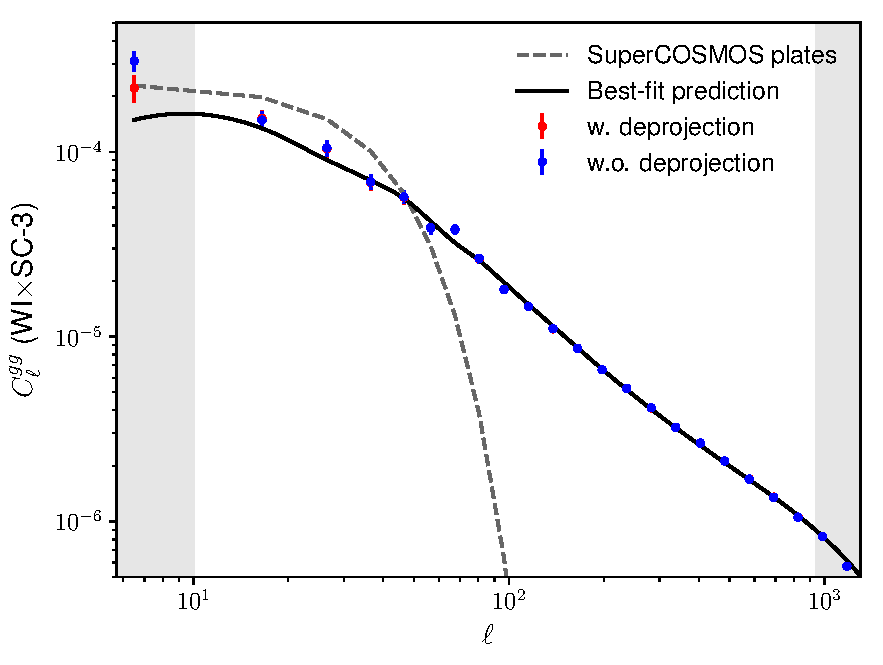
\includegraphics[width=0.48\textwidth]{./figures/cl_syst_summary.pdf}
      \caption{Fiducial redshift distributions of the different galaxy samples used in this analysis. See Table \ref{tab:z_bins} for further details.}
      \label{fig:clsyst}
    \end{figure}
    \subsubsection{Map-level deprojection}\label{sssec:methods.syst.deproj}
      For small levels of contamination, the impact of a given systematic on an observed sky map can be modelled at the linear level:
      \begin{equation}
        {\bf m}_{\rm obs}={\bf m}_{\rm true} + \epsilon\,{\bf t}.
      \end{equation}
      Here ${\bf m}_{\rm obs}$ and ${\bf m}_{\rm true}$ are vectors corresponding to the observed sky map and the true underlying quantity we wish to map respectively, ${\bf t}$ is a template map describing the contaminant (e.g. a map of the Galactic dust fluctuations), and $\epsilon$ is an unknown amplitude. In order to fully account for the effects of this contaminant one would build a likelihood for ${\bf m}_{\rm obs}$ using the equation above as a model (together with a model for ${\rm m}_{\rm true}$ and marginalize over $\epsilon$. As shown in \cite{2017MNRAS.465.1847E} and \cite{2019MNRAS.484.4127A}, within the pseudo-$C_\ell$ framework, this can be done exactly by projecting ${\bf m}_{\rm obs}$ onto the subspace perpendicular to ${\bf t}$ or, in other words, by ``deprojecting'' ${\bf t}$. The loss of modes due to deprojection then needs to be taken account when estimating the power spectrum, which can be done analytically.

      For our analysis, we deproject two systematic templates from the galaxy and $y$ maps. We create a reddening template using the dust map of \cite{1998ApJ...500..525S}, and remove its associated contamination from the $y$ maps and from all the galaxy overdensity maps. We also generate a star density template from the WISE data, and remove its associated fluctuations from all the galaxy overdensity maps.

    \subsubsection{$C_\ell$-level deprojection}\label{sssec:methods.syst.plates}
      We model the systematic fluctuations in the number density of sources in the \wisc sample caused by variations in the zero-point of the SuperCOSMOS photographic plate exposures as Gaussian random variations within the footprint of each exposure with a variance $\sigma^2_{\rm plate}$:
      \begin{equation}
        \delta_{\rm plate}(\nv) = \sum_p \delta_p\,S_{\rm plate}\,W(\nv-\nv_p),
      \end{equation}
      where $\delta_p$ is the fluctuation in exposure $p$ (with $\langle\delta_p^2\rangle=\sigma^2_{\rm plate}$, $S_{\rm plate}$ is the footprint area of each exposure and $W(\nv)$ is the plate window function. Assuming a roughly homogeneous coverage of the sky, the power spectrum of these fluctuations is given by
      \begin{equation}
        C_\ell^{\rm plate}=S_{\rm plate}\sigma_{\rm plate}^2\left|W_\ell\right|^2,
      \end{equation}
      where $W_\ell$ is the harmonic transform of the plate window function. SuperCOSMOS used photographic plates covering an area of $5^\circ\times5^\circ$. The corresponding window function can be roughly approximated as $|W_\ell|^2=\exp[-(\ell\,\theta_{\rm plate})^2/12]$, where $\theta_{\rm plate}=5\pi/180$ for 5-degree plates.
      
      The contamination from plate fluctuations can therefore be accounted for as an additive contribution to the model describing the galaxy auto-spectrum proportional to a template $T_\ell\equiv|W_\ell|^2$ with a free amplitude $A\equiv S_{\rm plate}\sigma_{\rm plate}^2$ that is marginalized over. Since $A$ is a linear parameter, this can be done analytically in a pre-processing step by modifying the inverse covariance matrix of the galaxy auto-spectra as follows \cite{1992ApJ...398..169R}:
      \begin{equation}
        {\sf Cov}^{-1}\hspace{6pt}\rightarrow\hspace{6pt} {\sf Cov}^{-1}-\frac{{\sf Cov}^{-1}{\bf T}\cdot{\bf T}^T{\sf Cov}^{-1}}{{\bf T}^T{\sf Cov}^{-1}{\bf T}},
      \end{equation}
      where ${\bf T}$ is a vector containing the template $T_\ell$ for all the scales used in the analysis.

    \subsubsection{Scale cuts}\label{sssec:methods.syst.scales}
      After deprojecting dust and stars at the map level, and the imprint of the SuperCOSMOS plates at the power spectrum level, we still observe an unacceptably large amount of power on scales $\ell<10$ in all galaxy auto-correlations involving \wisc. These may be due to residual star contamination that is not simply removed with a linear template, or To avoid biasing our results we therefore remove the lowest bandpower from these a
      
    \subsubsection{Redshift distribution uncertainties}\label{sssec:methods.syst.photoz}
      For each redshift bin we estimate fiducial redshift distributions using the method described in \cite{2018MNRAS.481.1133P}. In short, a true-redshift distribution is estimated from the distribution of photometric redshifts for a given bin using a model for the conditional photo-$z$ distribution:
      \begin{equation}
        p(z)=\int dz_{\rm photo}\,p(z|z_{\rm photo})\,p(z_{\rm photo}),
      \end{equation}
      where the model for $p(z|z_{\rm photo})$ was calibrated using overlapping spectroscopic data. Although the spectroscopic coverage of 2MPZ and \wisc is high compared to other photometric redshift surveys, the resulting redshift distributions are not infinitely precise, and therefore we need to account for any uncertainty in them that could affect our measurement.

      In particular, our interpretation of the $y\times \delta_g$ cross-correlation is especially sensitive to the width of the redshift distributions. This is because, while the amplitude to the galaxy auto-correlation is strongly affected by the width of the distribution (wider $p(z)$ reduce the clustering amplitude), whereas the cross-correlation with $y$ is almost insensitive to it. We therefore introduce an additional parameter $w_z$ that stretches the support of the redshift distribution while preserving unit total probability. Concretely, given a fiducial distribution $p_{\rm fid}(z)$ with mean redshift $\bar{z}$, $w_z$ is implemented as
      \begin{equation}
        p(z)\propto p_{\rm fid}\left(\bar{z}+\frac{z-\bar{z}}{w_z}\right),
      \end{equation}
      where the proportionality constant is fixed by making sure that $p(z)$ integrates to unity. We make $w_z$ a free parameter that we marginalize over with a top-hat prior $0.8<w_z<1.2$, which is broader than the actual uncertainty on the distribution widths from photo-$z$ calibration \todo{It would be really good to make this statement more quantitative}.

  \subsection{Likelihood}\label{ssec:methods.like}
    In order to connect our measurements with the posterior distribution of the model parameters $\vec{\theta}$, we assume that the measured power spectra follow a Gaussian likelihood:
    \begin{equation}
      -2\log p({\bf d}|\vec{\theta}) = \chi^2\equiv ({\bf d}-{\bf t}(\vec{\theta}))^T {\sf C}^{-1} ({\bf d}-{\bf t}(\vec{\theta})),
    \end{equation}
    where ${\bf d}$ is a vector of power spectrum measurements, ${\bf t}(\vec{\theta})$ is the theory prediction for ${\bf d}$ with parameters $\vec{\theta}$ and ${\sf Cov}$ is the covariance matrix described in the previous section.

    We explore the likelihood of each redshift bin separately. For each redshift bin, our data vector ${\bf d}$ includes two sets of power spectrum measurements, corresponding to the auto-correlation of the galaxy overdensity and to its cross-correlation with the Compton-$y$ map, ${\bf d}=(C^{gg}_\ell,C^{gy}_\ell)$. We compute all power spectra in the range of multipoles $2<\ell<1024$, binned into the bandpowers described in Table \TODO{make table}. For a given redshift bin $b$ with mean redshift $\bar{z}_b$, we use only multipoles $\ell<\ell^b_{\rm max}\equiv k_{\rm max}\,\chi(\bar{z}_b)-1/2$, where $k_{\rm max}=1\,{\rm Mpc}^{-1}$. As described in Section \ref{ssec:results.syst}, we also remove the first bandpower $(\ell\lesssim10)$ from all the galaxy auto-spectra for the WI$\times$SC redshift bins.

    For each redshift bin, our theory model has five free parameters: $\log_{10}M_{\rm min}/M_\odot$, $\log_{10}M_1'/M_\odot$, $1-b_{\rm H}$, $\rho_{yg}$, and a nuisance width parameter $w_z$. The first two parameters effectively fit the galaxy bias and small-scale amplitude in the galaxy auto-correlation, while $1-b_{\rm H}$ and $\rho_{yg}$ are then constrained by including the tSZ cross-correlation. We fix all cosmological parameters to the best-fit values in \TODO{check with Nick where the parameters were obtained}: $(\Omega_c h^2,\Omega_bh^2,h,\sigma_8,n_s)=(0.119,0.0224,0.6766,0.8102,0.9556)$. We impose the following top-hat priors on the free parameters:
    \begin{align}
      &10\le\log_{10}M_{\rm min}/M_\odot\le16,\\
      &10\le\log_{10}M_1'/M_\odot\le16,\\
      &0\le(1-b_H)\le0.99,\\
      &-1\le\rho_{yg}\le1,\\
      &0.8\le w_z\le1.2.
    \end{align}
    We sample the resulting posterior distributions using the Markov chain Monte Carlo method (MCMC) as implemented in the {\tt emcee} software package \citep{2013PASP..125..306F}\footnote{\url{https://emcee.readthedocs.io/en/v2.2.1/}.}.
  
\section{Results}\label{sec:results}
  \begin{enumerate}
    \item Fiducial results
    \item Constant fit
    \item $\langle bP_e\rangle$
    \item Derive anything from the above?
    \item Systematics:
    \begin{itemize}
      \item CIB
      \item NILC
      \item 
    \end{itemize}
  \end{enumerate}

  \subsection{Power spectra and covariances}\label{ssec:results.cls}
    We estimate the galaxy auto-power spectrum, the galaxy-tSZ cross-spectrum, and their covariance matrix for each of the redshift bins shown in Figure \ref{fig:dndz} using the methods described in Section \ref{sec:methods}. The resulting measured power spectra and errors are shown in red in Figure \ref{fig:cls}, together with their best-fit halo model prediction in black, decomposed into its 1-halo and 2-halo contributions (green and grey respectively). The bottom part of each panel shows the residuals with respect to the best-fit prediction normalized by the 1$\sigma$ errors. The grey bands cover the data points not used in the analysis due to scale cuts.
    
    Figure \ref{fig:covs} shows the correlation matrix of the combined data vector $(C^{gg}_\ell,C^{gy}_\ell)$ for each redshift bin (where the correlation matrix $r_{ij}$ is related to the covariance $C_{ij}$ as $r_{ij}=C_{ij}/\sqrt{C_{ii}C_{jj}}$). At low redshifts, 2MPZ shows strong correlations between different scales, mostly caused by the non-Gaussian contribution to the covariance matrix (Eq. \ref{eq:cov_ng}). These become less relevant at higher redshifts, where non-linear effects are weaker, and where the radial projection pushes the non-linear scale into larger multipole values.
    
    Overall, we find a good agreement between theory and data over the scales used in this analysis. We discuss this agreement and the associated scientific results in the following sections.

  \subsection{Fiducial results}\label{ssec:results.fid}
    
    
    \TODO{Describe fiducial measurement of $(1-b)$ from 2MPZ $+$ WISC, using whatever mass function was used for the Planck clusters analysis.}
    \TODO{Discuss these results: is it compatible with a constant, discuss mass dependence (from SZ source masking), translate into $\langle bP_e \rangle$ and place in context of existing measurements.}

  \subsection{Systematics analysis}\label{ssec:results.syst}
    \subsubsection{Large-scale galaxy clustering systematics}\label{sssec:results.syst.gg}
      \TODO{Describe different efforts to understand/mitigate/remove systematics in WISC (removing first point, fitting for $C_\ell$ template, template deprojection of stars and other stuff).}
      \TODO{Compare with SDSS results if available}
    \subsubsection{Photometric redshift systematics}\label{sssec:results.syst.pz}
      \TODO{Compare results with different $N(z)$ choices.}
    \subsubsection{tSZ contamination}\label{sssec:results.syst.y}
      \TODO{Compare results with NILC map}
      \TODO{Quantify CIB contamination}

  \begin{figure*}
    \centering
    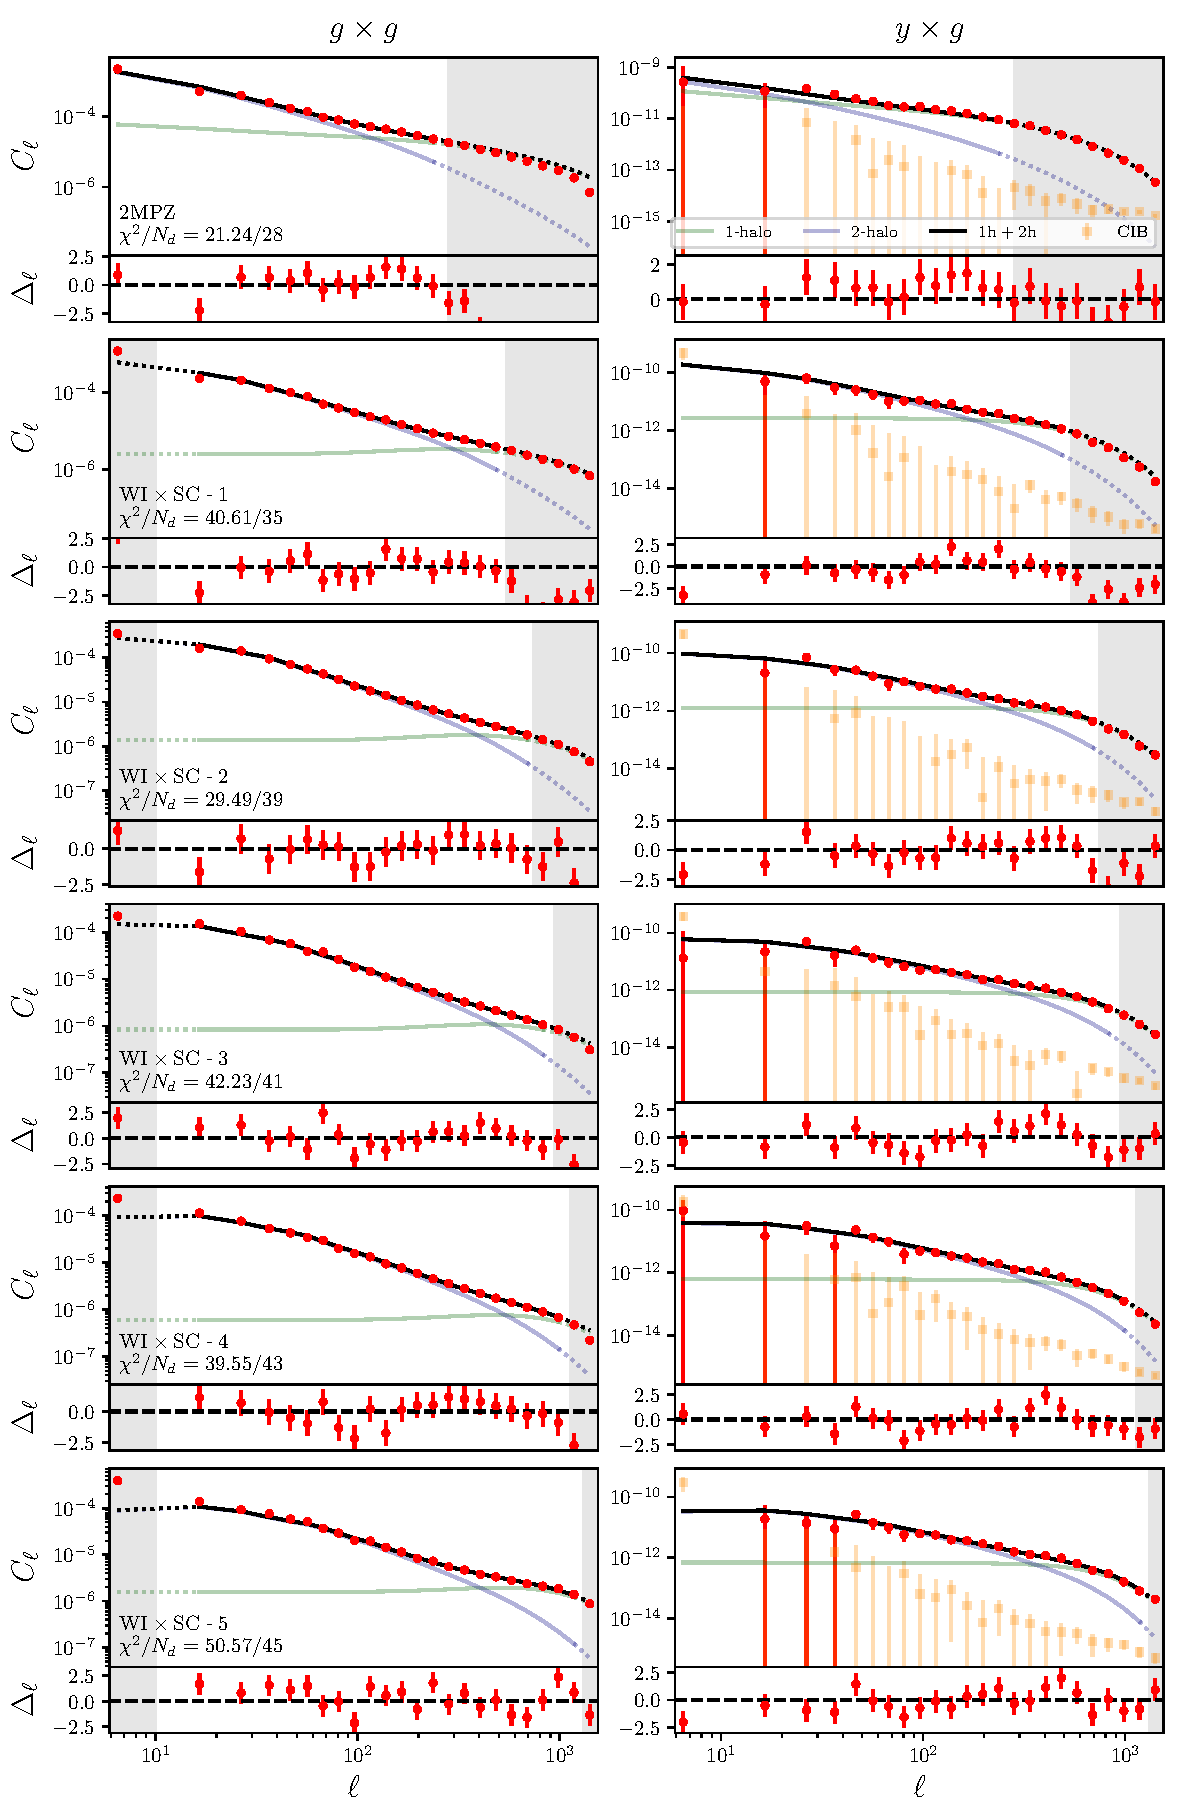
\includegraphics[width=0.8\textwidth]{./figures/fits.pdf}
    \caption{Redshift distributions assumed for the Gaussian simulations used in this analysis.}
    \label{fig:cls}
  \end{figure*}
  \begin{figure*}
    \centering
    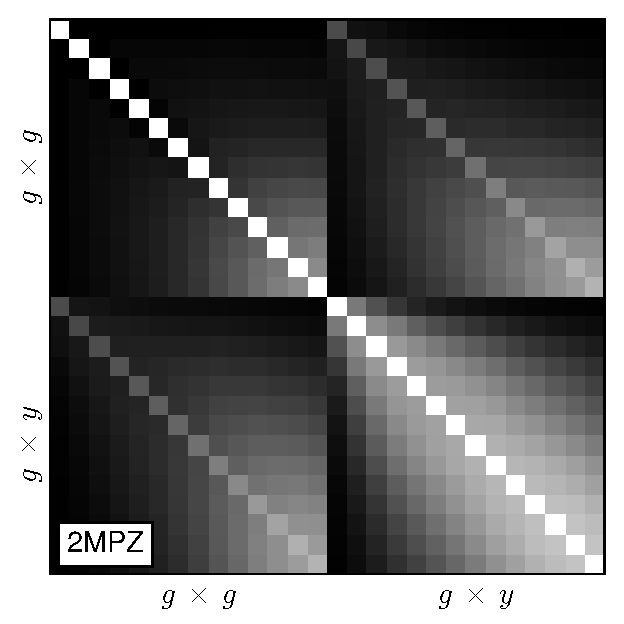
\includegraphics[width=0.3\textwidth]{./figures/cov_2mpz.pdf}
    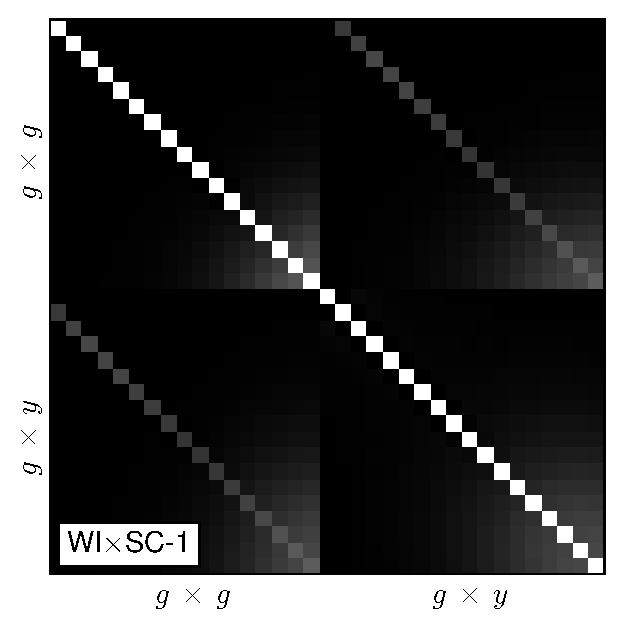
\includegraphics[width=0.3\textwidth]{./figures/cov_wisc1.pdf}
    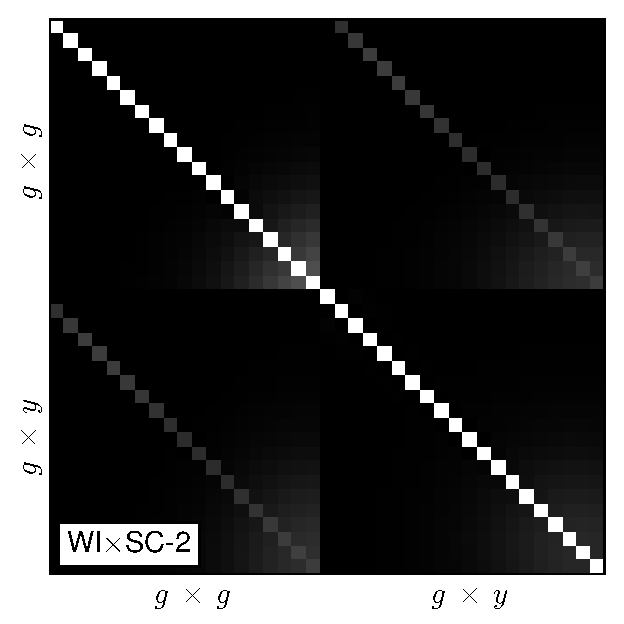
\includegraphics[width=0.3\textwidth]{./figures/cov_wisc2.pdf}
    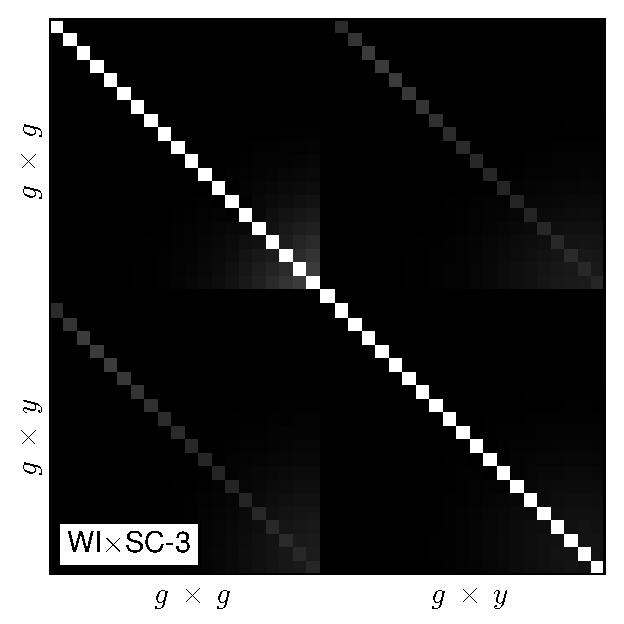
\includegraphics[width=0.3\textwidth]{./figures/cov_wisc3.pdf}
    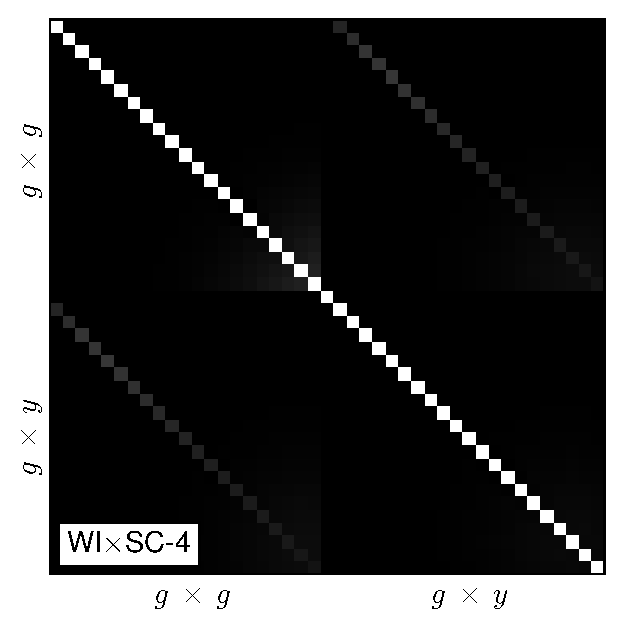
\includegraphics[width=0.3\textwidth]{./figures/cov_wisc4.pdf}
    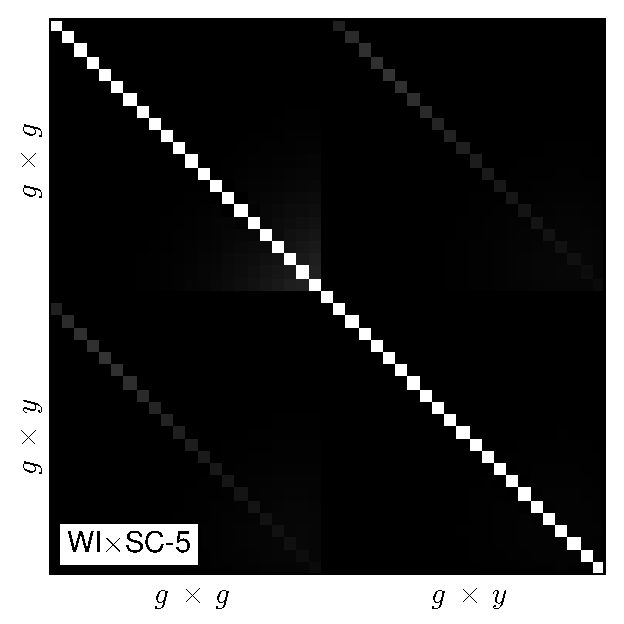
\includegraphics[width=0.3\textwidth]{./figures/cov_wisc5.pdf}
    \caption{Redshift distributions assumed for the Gaussian simulations used in this analysis.}
    \label{fig:covs}
  \end{figure*}
  \begin{figure}
    \centering
    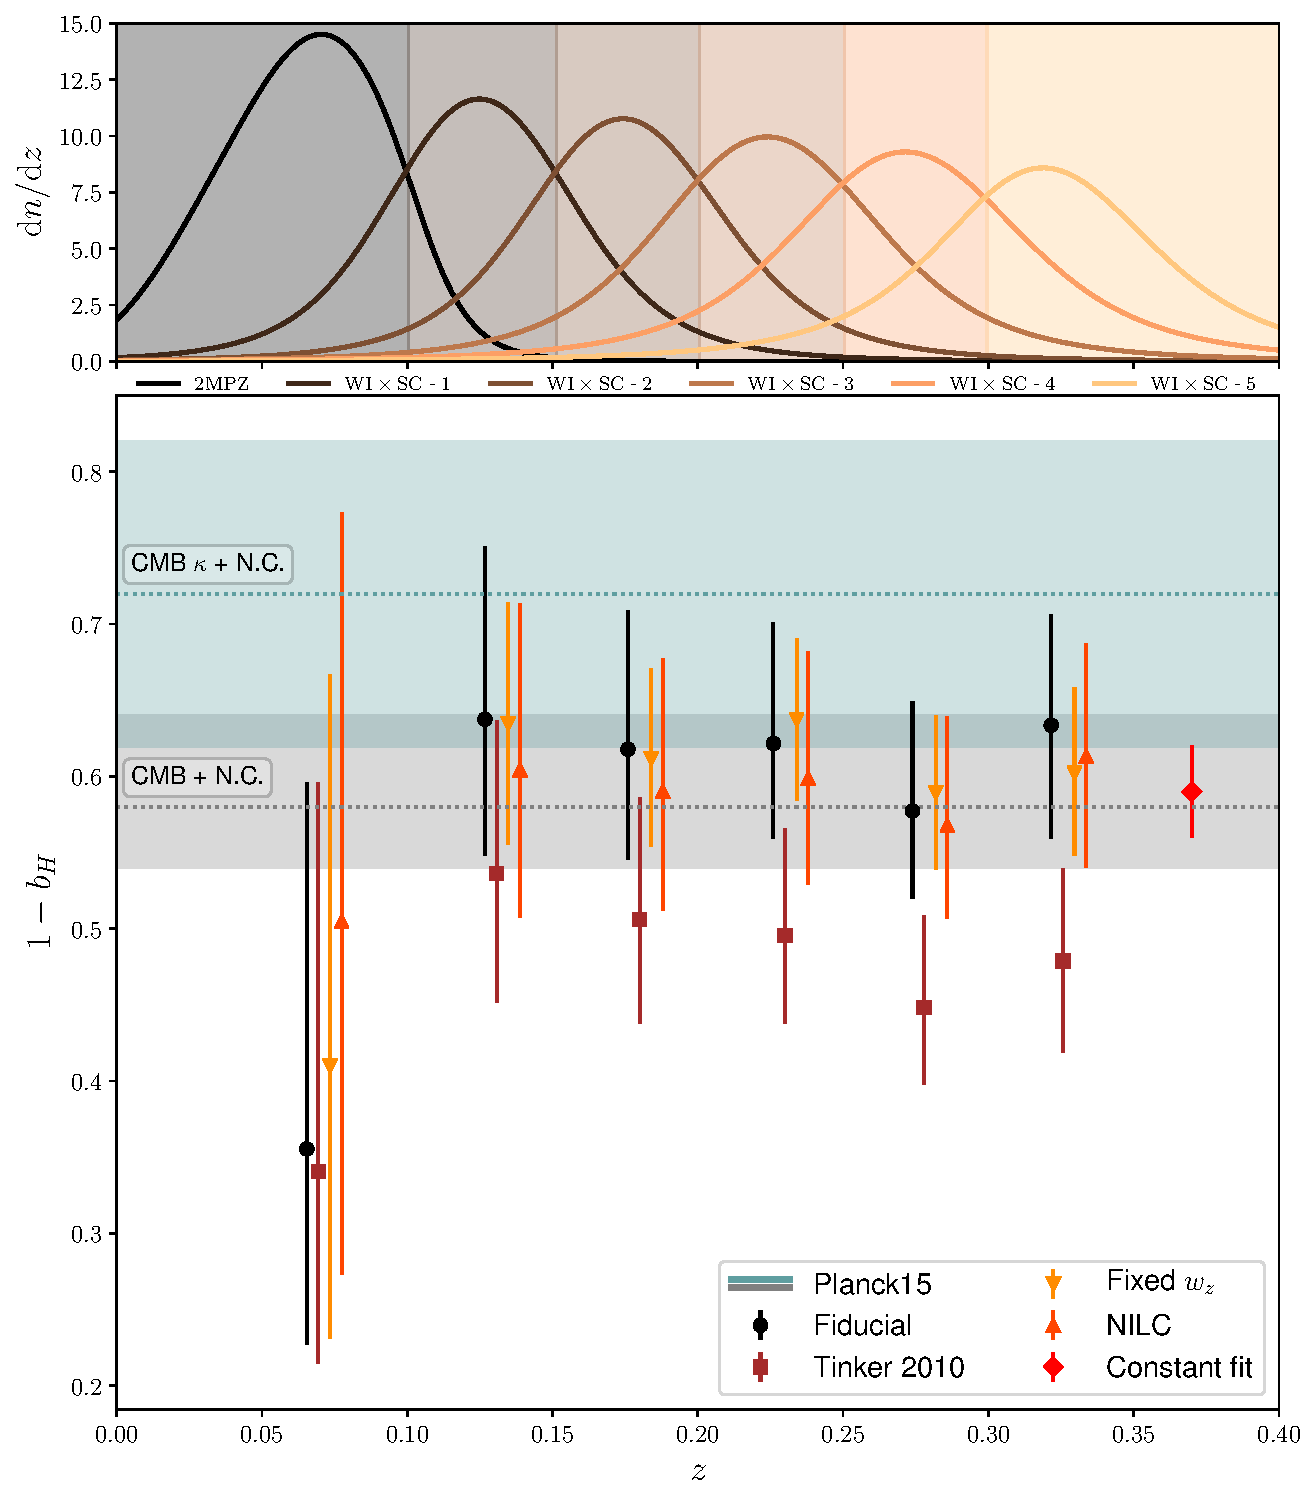
\includegraphics[width=0.5\textwidth]{./figures/bhydro.pdf}
    \caption{Redshift distributions assumed for the Gaussian simulations used in this analysis.}
    \label{fig:bh}
  \end{figure}
  \begin{figure}
    \centering
    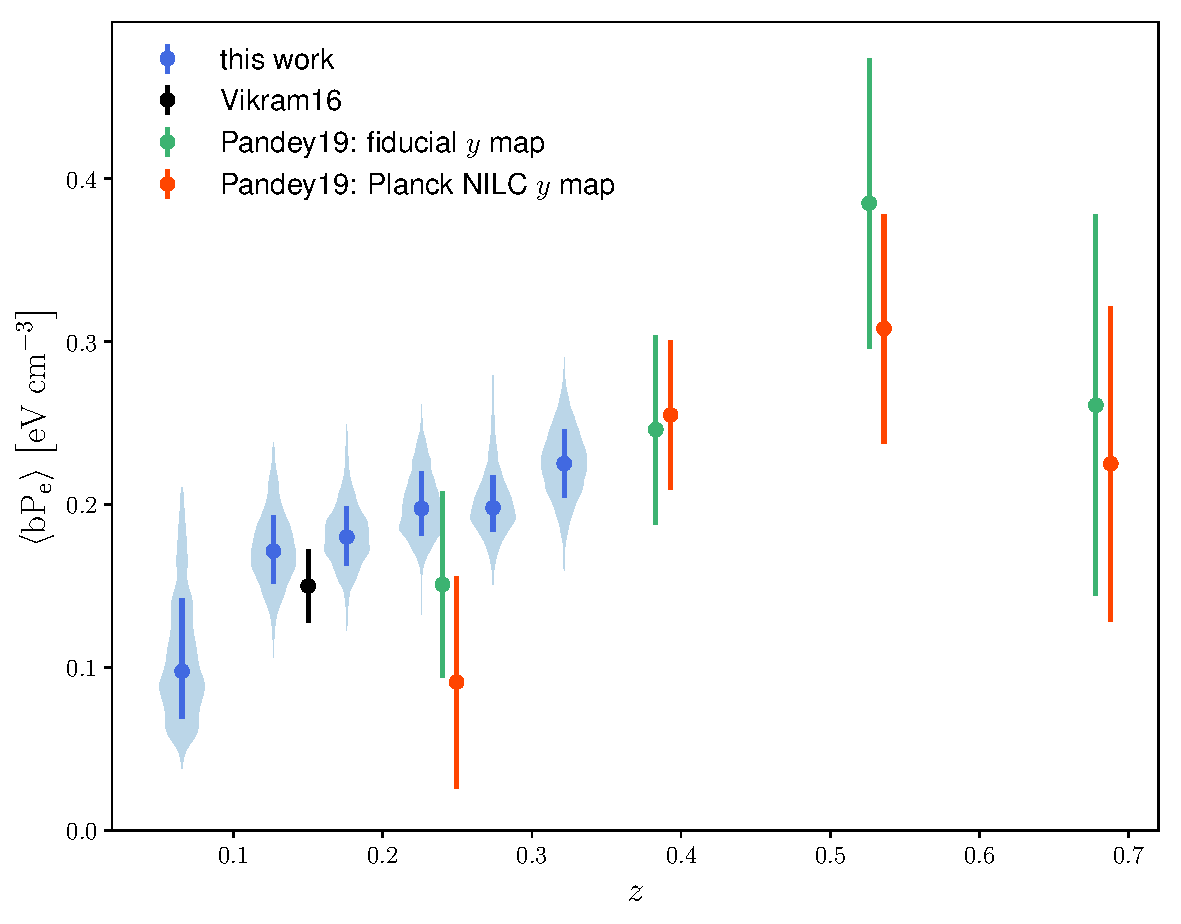
\includegraphics[width=0.5\textwidth]{./figures/by.pdf}
    \caption{Redshift distributions assumed for the Gaussian simulations used in this analysis.}
    \label{fig:by}
  \end{figure}
  \begin{figure*}
    \centering
    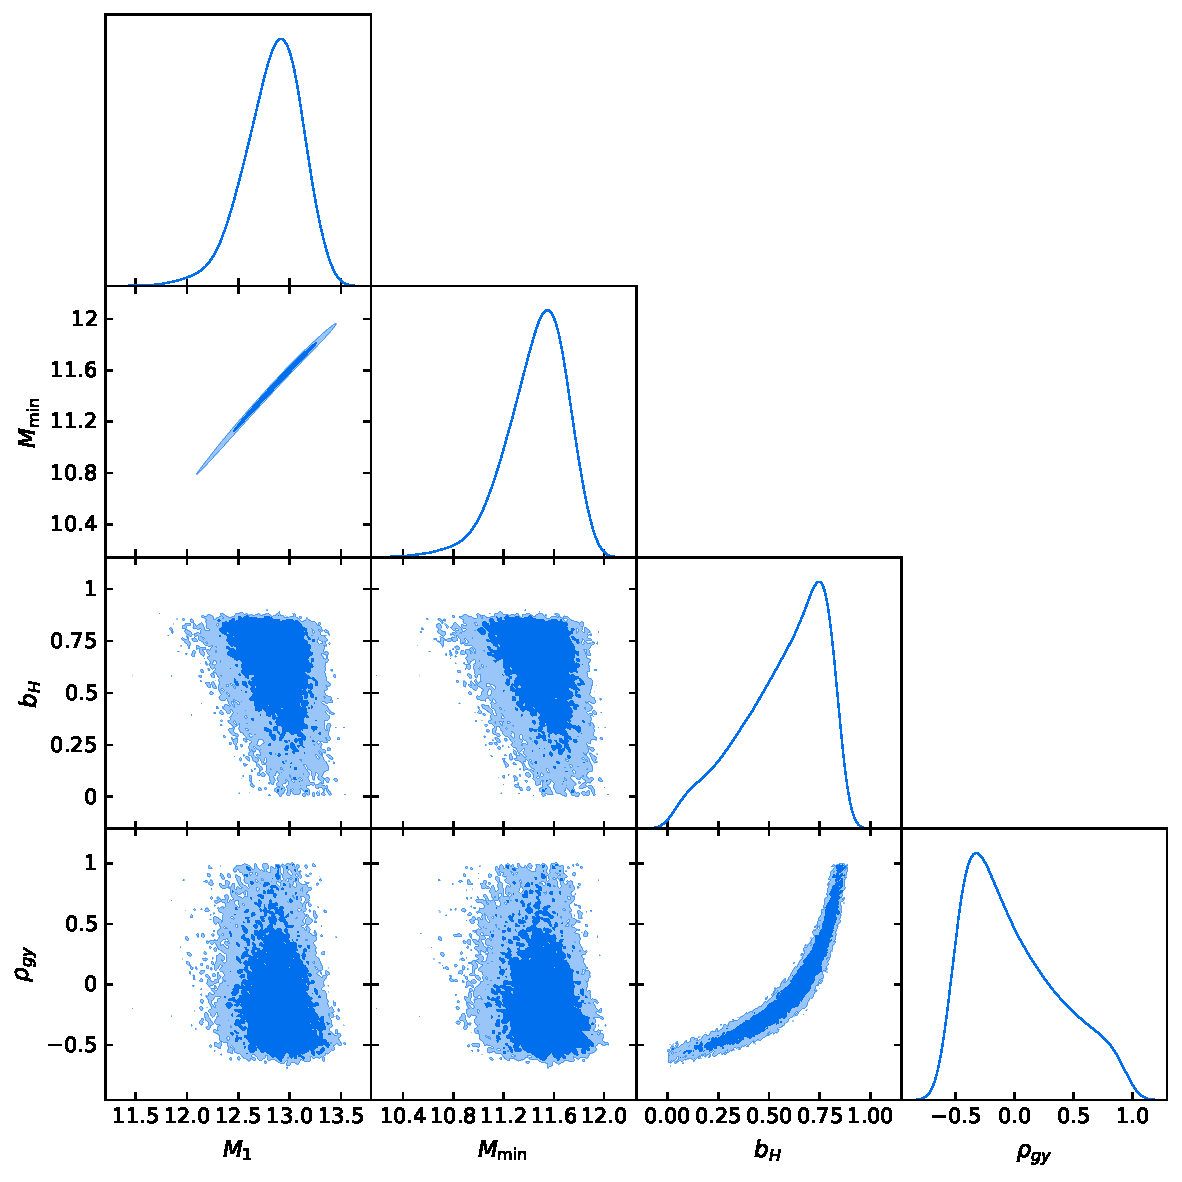
\includegraphics[width=0.47\textwidth]{./figures/fiducial_2mpz.pdf}
    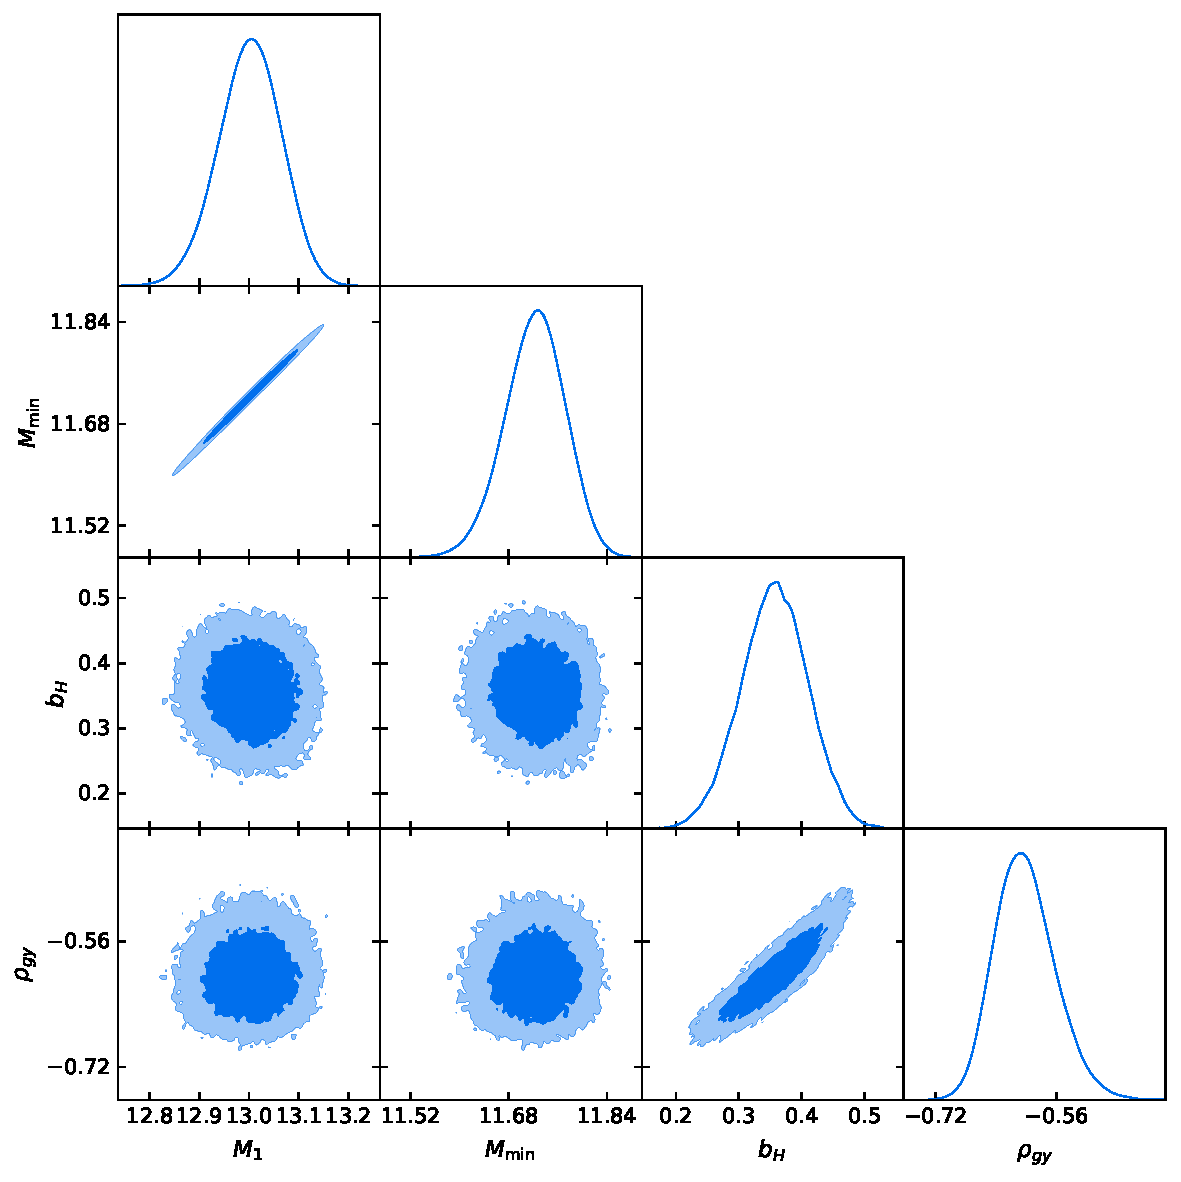
\includegraphics[width=0.47\textwidth]{./figures/fiducial_wisc3.pdf}
    \caption{Redshift distributions assumed for the Gaussian simulations used in this analysis.}
    \label{fig:triangle}
  \end{figure*}

\section{Discussion}\label{sec:discussion}
  \lipsum[2]

\section*{Acknowledgements}
  We thank Thor the almighty and the Beach Boys for useful comments and discussions. DA acknowledges support from the Beecroft trust and from the Science and Technology Facilities Council (STFC) through an Ernest Rutherford Fellowship, grant reference ST/P004474/1.
  
\setlength{\bibhang}{2.0em}
\setlength\labelwidth{0.0em}
\bibliography{paper}

\appendix
%\onecolumngrid
\section{An appendix}\label{app:app}
  \lipsum[3]

\end{document}
